\documentclass[12pt]{beamer}

\parindent 0mm
\parskip 0.5em plus 1pt

%\usetheme{Darmstadt}
%\usetheme{Marburg}
%\usetheme{Hannover}
%\usecolortheme{crane}
\usefonttheme[onlylarge]{structurebold}
\setbeamerfont*{frametitle}{size=\normalsize,series=\bfseries}
\setbeamertemplate{navigation symbols}{}
\addtobeamertemplate{navigation symbols}{}{%
    \usebeamerfont{footline}%
    \usebeamercolor[fg]{footline}%
    \hspace{1em}%
    \insertframenumber/\inserttotalframenumber
}

\usepackage[czech]{babel}
\usepackage[utf8]{inputenc}
\usepackage{times}
\usepackage[T1]{fontenc}
\usepackage{wrapfig}

% Setup TikZ
\usepackage{tikz}
\usetikzlibrary{arrows}
\tikzstyle{block}=[draw opacity=0.7,line width=1.4cm]
\usepackage{amssymb}
\usepackage{amsthm}
\usepackage{amscd}
\usepackage{wasysym}
\usepackage{verbatim}
\usepackage{euler,eucal}
%\newcommand{\slideCite}[1]{\raisebox{1ex}{\tiny \cite{#1}}}


\newtheorem{define}{Definice}[section]
\newtheorem*{define*}{Definice}
\newtheorem{veta}[define]{Věta}
\newtheorem*{veta*}{Věta}
\newtheorem{remark}[define]{Poznámka}

%% moje nastaveni
\newcommand{\nazev}{Model hromadné obsluhy}
\newcommand{\nazevsl}{\nazev}

\newcommand{\matice}{\mathbb}
\newcommand{\Tr}{\mbox{Tr~}}

\DeclareMathOperator{\Diam}{Diam}
\DeclareMathOperator{\Area}{Area}
\DeclareMathOperator{\cotg}{cotg}

%% MARK: Title & Data
\title%[Finding structures in graphs]
{
    \includegraphics[width=0.25\columnwidth]{imgs/fjfi.png}\\
    \nazev
}

\author[Zikmund]
{
    Tomáš~Zikmund
}

\institute[FJFI CVUT]
{
    tomaszikmund@me.com
    \and
    Fakulta jaderná a fyzikálně inženýrská, Břehová 7, 115 19 Praha 1
}

\date{MMC -- \today}

%% Begin Document
\begin{document}

    \begin{frame}
        \titlepage
    \end{frame}

    \begin{frame}{Obsah}
        \tableofcontents
    \end{frame}

    %% MARK: Introduction
    \section{Motivace}
    \begin{frame}{Motivace}
	Jaký je minimální počet pokladních, 
    aby bylo obslouženo co nejvíce zákazníků?
\end{frame}





    \section{Modely hromadné obsluhy}
    \begin{frame}{Modely hromadné obsluhy}
\begin{block}{Poissonovo rozdělení}
\[P(X = x) = \frac{\lambda^k}{k!}\exp(-\lambda).\]
\(\lambda\)\ldots střední hodnota počtu událostí
\end{block}
\begin{block}{Exponenciální rozdělení}
\[f(x) = \lambda \exp(-\lambda x),\qquad\mbox{pro~}x\geq 0.\]
\(\frac{1}{\lambda}\)\ldots střední hodnota doby mezi událostmi
\end{block}
\end{frame}

\begin{frame}{Model s diskrétním časem}
	\begin{figure}[h]
\setlength{\unitlength}{0.99\columnwidth}
\begin{picture}(1,0.322)
\put(0,0.1){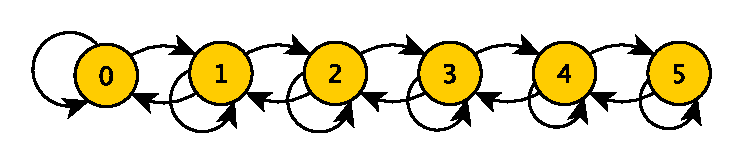
\includegraphics[width=\unitlength]{imgs/markowski.pdf}}
\small
\put(0,0.12){\rotatebox{90}{$1-\lambda\cdot\Delta t$}}
\put(0.17,0.28){$\lambda\cdot\Delta t$}
\put(0.10,0.10){\rotatebox{45}{$\mu\cdot\Delta t$}}
\put(0.33,0.28){$\lambda\cdot\Delta t$}
\put(0.29,0.09){\rotatebox{45}{$2\mu\cdot\Delta t$}}
\put(0.49,0.28){$\lambda\cdot\Delta t$}
\put(0.45,0.08){\rotatebox{45}{$3\mu\cdot\Delta t$}}
\put(0.65,0.28){$\lambda\cdot\Delta t$}
\put(0.60,0.08){\rotatebox{45}{$3\mu\cdot\Delta t$}}
\put(0.81,0.28){$\lambda\cdot\Delta t$}
\put(0.75,0.08){\rotatebox{45}{$3\mu\cdot\Delta t$}}
%\tiny
%\footnotesize
\scriptsize
\put(0.11,0.030){\rotatebox{45}{$1-(\mu+\lambda)\Delta t$}}
\put(0.27,0.016){\rotatebox{45}{$1-(2\mu+\lambda)\Delta t$}}
\put(0.44,0.014){\rotatebox{45}{$1-(3\mu+\lambda)\Delta t$}}
\put(0.59,0.020){\rotatebox{45}{$1-(3\mu+\lambda)\Delta t$}}
\put(0.74,0.020){\rotatebox{45}{$1-(3\mu+\lambda)\Delta t$}}
\Huge
\put(0.97,0.225){\ldots}
\normalsize
\end{picture}
\caption{Fronta THO jako markovský proces. Zákazníci přicházejí s paramtrem \(\lambda\) 
a můžou být obslouženi u jedné ze 3 přepážek. Doba obsluhy je popsána parametrem \(\mu\). 
Délka fronty jsou jednotlivé stavy markovského procesu. }
\label{fig:markowski}
\end{figure}
\end{frame}

\begin{frame}{Model s diskrétním časem}
\begin{itemize}
	\item čas simulace \(T\) na \(M\) poditervalů délky \(\Delta t\)
    \item \(\Delta t\) tak, že \(P[X\geq 2] \approx 0\)
    \item velmi jednoduchý, ale neefektivní
\end{itemize}
\end{frame}

\begin{frame}{Model s diskrétními událostmi}
\begin{figure}
\definecolor{ffqqqq}{rgb}{1.,0.,0.}
\definecolor{qqzzff}{rgb}{0.,0.6,1.}
\definecolor{qqqqff}{rgb}{0.,0.,1.}
\definecolor{cqcqcq}{rgb}{0.7529411764705882,0.7529411764705882,0.7529411764705882}
\begin{tikzpicture}[line cap=round,line join=round,>=triangle 45,x=0.3cm,y=0.8cm]
\draw [color=cqcqcq,, xstep=1.5cm,ystep=0.8cm] (0,-7.5) grid (32,0.5);
\draw[->,color=black] (-3.,0.) -- (32,0.);
\foreach \x in {,5.,10.,15.,20.,25.,30.}
\draw[shift={(\x,0)},color=black] (0pt,2pt) -- (0pt,-2pt) node[above] {\footnotesize $\x$};
\draw[<-,color=black] (0.,-7.5) -- (0.,0.5);
\foreach \y in {7.,6.,5.,4.,3.,2.,1.}
\draw[shift={(0,-\y)},color=black] (2pt,0pt) -- (-2pt,0pt) node[left] {\footnotesize $\y$};
\draw[color=black] (0pt,-10pt) node[right] {\footnotesize $0$};
\clip(-3.,-8.5) rectangle (46.010087437351785,0.507536612606849);
\draw [line width=4.pt,color=qqzzff] (1.8,-1.)-- (11.,-1);
\draw [line width=4.pt,color=qqzzff] (3.9,-2.)-- (13.,-2.);
\draw [line width=4.pt,color=qqzzff] (8.,-3.)-- (16.,-3.);
\draw [line width=3.2pt,color=ffqqqq] (9.2,-4.)-- (11.,-4.);
\draw [line width=4.pt,color=qqzzff] (15.,-5.)-- (22.,-5);
\draw [line width=4.pt,color=qqzzff] (11.,-4.)-- (20.,-4.);
\draw [line width=3.2pt,color=ffqqqq] (15.8,-6.)-- (20.,-6.);
\draw [line width=4.pt,color=qqzzff] (20.,-6.)-- (26.,-6.);
\draw [line width=3.2pt,color=ffqqqq] (18.,-7.)-- (22.,-7.);
\draw [line width=4.pt,color=qqzzff] (22.,-7.)-- (29.5,-7.);
\begin{scriptsize}
\draw [fill=qqqqff] (1.8,-1.) circle (2.5pt);
\draw[color=qqqqff] (2.4284789958647366,-0.6376375884262001) node {$A$};
\draw [fill=qqqqff] (3.9,-2.) circle (2.5pt);
\draw[color=qqqqff] (4.463417911420552,-1.644601110024226) node {$B$};
\draw [fill=qqqqff] (8.,-3.) circle (2.5pt);
\draw[color=qqqqff] (8.618084864013674,-2.6515646316222523) node {$C$};
\draw [fill=qqqqff] (9.2,-4.) circle (2.5pt);
\draw[color=qqqqff] (9.805132564754567,-3.6387837704438466) node {$D$};
\draw [fill=qqqqff] (15.,-5.) circle (2.5pt);
\draw[color=qqqqff] (15.570792825496044,-4.6457472920418725) node {$E$};
\draw [fill=qqqqff] (15.8,-6.) circle (2.5pt);
\draw[color=qqqqff] (16.418684040310968,-5.6527108136398985) node {$F$};
\draw [fill=qqqqff] (18.,-7.) circle (2.5pt);
\draw[color=qqqqff] (18.62320119882977,-6.639929952461492) node {$G$};
\end{scriptsize}
% casovy krok
\only<1>{\draw [line width=1.4pt,color=ffqqqq] (1.8,0.)-- (1.8,-7.5)};
\only<2>{\draw [line width=1.4pt,color=ffqqqq] (3.9,0.)-- (3.9,-7.5)};
\only<3>{\draw [line width=1.4pt,color=ffqqqq] (8,0.)-- (8,-7.5)};
\only<4>{\draw [line width=1.4pt,color=ffqqqq] (9,0.)-- (9,-7.5)};
\only<5>{\draw [line width=1.4pt,color=ffqqqq] (11,0.)-- (11,-7.5)};
\only<6>{\draw [line width=1.4pt,color=ffqqqq] (13,0.)-- (13,-7.5)};
\only<7>{\draw [line width=1.4pt,color=ffqqqq] (15,0.)-- (15,-7.5)};
\only<8>{\draw [line width=1.4pt,color=ffqqqq] (15.8,0.)-- (15.8,-7.5)};
\only<9>{\draw [line width=1.4pt,color=ffqqqq] (13,0.)-- (13,-7.5)};
\only<10>{\draw [line width=1.4pt,color=ffqqqq] (18,0.)-- (18,-7.5)};
\only<11>{\draw [line width=1.4pt,color=ffqqqq] (20,0.)-- (20,-7.5)};
\only<12>{\draw [line width=1.4pt,color=ffqqqq] (22,0.)-- (22,-7.5)};
\only<13>{\draw [line width=1.4pt,color=ffqqqq] (26,0.)-- (26,-7.5)};
\only<14>{\draw [line width=1.4pt,color=ffqqqq] (29.5,0.)-- (29.5,-7.5)};
\end{tikzpicture}
\end{figure}
\end{frame}

\begin{frame}{Ustálený stav}
\[\forall k \qquad p_k = \lim_{t\to\infty} p_k(t)\]
\(p_k\)\ldots počet zákazníků v pekárně
\begin{itemize}
	\item Nutná podmínka: \[\lambda < n\mu \]
\end{itemize}
\end{frame}
\begin{frame}{Ustálený stav}
\begin{figure}
\centering
\includegraphics[width=0.8\columnwidth]{imgs/fronta.pdf}
\label{fig:fronta}
\caption{Vývoj počtu zákazník ve frontě v průběhu 16 hodin. Fronta je bez omezení, vstupní tok \(\lambda = 100 \mbox{~h}^{-1}\). }
\end{figure}
\end{frame} 

    \section{Model pekárny}
    \begin{frame}{Model pekárny}
    \begin{block}{Vstupní tok}
    Do pekárny přicházejí zákazníci (\(\lambda =\)zákazníci za hodinu)
    \end{block}
    \begin{block}{Výstupní tok}
    \begin{itemize}
    \item počet pokladen
    \item střední doba obsluhy (\(\frac{\Delta t}{\mu}\))
    \end{itemize}
    \end{block}
    \begin{block}{Fronta}
    \begin{itemize}
    \item nekonečná
    \item FIFO
    \item střední doba trpělivosti (\(\tau\))
    \end{itemize}
    \end{block}
\end{frame}
\begin{frame}{Jedna realizace}
    \begin{figure}
\centering
\includegraphics[width=0.8\columnwidth]{imgs/jedenPrubeh.pdf}
\label{fig:jedenPrubeh}
\caption{Simulace jedné osmihodinové směny v pekárně s jednou pokladnou.}
\end{figure}
\end{frame}
\begin{frame}{Jedna realizace}
    \begin{figure}
\centering
\includegraphics[width=0.8\columnwidth]{imgs/jedenPrubeh4.pdf}
\label{fig:jedenPrubeh4}
\caption{Simulace jedné osmihodinové směny v pekárně se 4 pokladnami.}
\end{figure}
\end{frame}

    
    \section{Výsledky}
    \begin{frame}{Výsledky}
	Simulace:
	\begin{itemize}
    \item s frontou bez omezení
    \item s omezenou frontou na 20 zákazníků
    \item s frontou bez omezení, trpělivost zákazníků \(\sim 20\) minut
	\end{itemize}
\end{frame}

\begin{frame}{Simulace s neomezenou frontou}
	\begin{figure}
	\includegraphics[width=0.99\columnwidth]{imgs/bezOmezeni.pdf}
    %\caption{\(\Gamma_{100}(u), \qquad u_n = 2\sqrt{17} n\)}
	\end{figure}
\end{frame}
\begin{frame}{Simulace s neomezenou frontou}
\small
	\begin{tabular}{c|r@{$\pm$}l|r@{$\pm$}l|r@{$\pm$}l|r@{$\pm$}l}
	\#  & \multicolumn{2}{|c|}{Tržba} & \multicolumn{2}{|c|}{Doba čekání} & \multicolumn{2}{|c|}{Odmítnutí zák.} & \multicolumn{2}{|c}{Délka fronty}\\ \hline\hline	
	1 &   24000 & 2000  &  168     &  7      &  560   & 30    &  280    & 20    \\
	2 &   48000 & 2000  &   97     &  9      &  320   & 33    &  160    & 20    \\
	3 &   71000 & 2000  &   30     & 10      &   80   & 36    &   40    & 20    \\
	4 &   79000 & 3000  &    1.9   &  0.9    &    4   &  6    &    3    &  2    \\
	5 &   80000 & 3000  &    0.4   &  0.1    &    0   &  2    &    0.6  &  0.2  \\
	6 &   80000 & 3000  &    0.11  &  0.05   &    0   &  1    &    0.18 &  0.08 \\
	7 &   80000 & 3000  &    0.03  &  0.02   &    0.1 &  0.5  &    0.05 &  0.03 \\
	8 &   80000 & 3000  &    0.008 &  0.007  &    0.0 &  0.3  &    0.01 &  0.01 
\end{tabular}
\end{frame}


\begin{frame}{Simulace s neomezenou frontou}
	\begin{figure}
	\includegraphics[width=0.99\columnwidth]{imgs/maxFronta.pdf}
    %\caption{\(\Gamma_{100}(u), \qquad u_n = 2\sqrt{17} n\)}
	\end{figure}
\end{frame}
\begin{frame}{Simulace s neomezenou frontou}
\small
\begin{tabular}{c|r@{$\pm$}l|r@{$\pm$}l|r@{$\pm$}l|r@{$\pm$}l}
	\#  & \multicolumn{2}{|c|}{Tržba} & \multicolumn{2}{|c|}{Doba čekání} & \multicolumn{2}{|c|}{Odmítnutí zák.} & \multicolumn{2}{|c}{Délka fronty}\\ \hline\hline	
	1 &   24000 & 2000  &   11.4   &  0.4    &  560   & 30    &  19.2  & 0.1  \\
	2 &   48000 & 2000  &   10.6   &  0.3    &  320   & 40    &  17.8  & 0.4  \\
	3 &   71000 & 2000  &    8     &  1      &   90   & 33    &  13    & 2    \\
	4 &   80000 & 3000  &    1.7   &  0.5    &    5   &  6    &   3    & 1    \\
	5 &   80000 & 3000  &    0.4   &  0.2    &    0   &  1    &   0.7  & 0.3  \\
	6 &   80000 & 3000  &    0.11  &  0.06   &    0   &  1    &   0.2  & 0.1  \\
	7 &   80000 & 3000  &    0.03  &  0.02   &    0.0 &  0.3  &   0.05 & 0.03 \\
	8 &   80000 & 3000  &    0.010 &  0.009  &    0.0 &  0.1  &   0.02 & 0.01 
\end{tabular}
\end{frame}


\begin{frame}{Simulace s neomezenou frontou}
	\begin{figure}
	\includegraphics[width=0.99\columnwidth]{imgs/timeout.pdf}
    %\caption{\(\Gamma_{100}(u), \qquad u_n = 2\sqrt{17} n\)}
	\end{figure}
\end{frame}
\begin{frame}{Simulace s neomezenou frontou}
\small
\begin{tabular}{c|r@{$\pm$}l|r@{$\pm$}l|r@{$\pm$}l|r@{$\pm$}l}
	\#  & \multicolumn{2}{|c|}{Tržba} & \multicolumn{2}{|c|}{Doba čekání} & \multicolumn{2}{|c|}{Odmítnutí zák.} & \multicolumn{2}{|c}{Délka fronty}\\ \hline\hline	
	1 &   24000 & 2000  &   10.1  &  0.5   &  560 & 30  &  17    & 1    \\
	2 &   48000 & 2000  &    5.8  &  0.6   &  320 & 40  &  10    & 1    \\
	3 &   71000 & 2000  &    2.3  &  0.4   &  130 & 30  &   3.9  & 0.8  \\
	4 &   75000 & 2000  &    0.8  &  0.2   &   50 & 10  &   1.4  & 0.4  \\
	5 &   79000 & 3000  &    0.3  &  0.08  &   15 &  6  &   0.5  & 0.1  \\
	6 &   79000 & 2000  &    0.09 &  0.04  &    5 &  3  &   0.15 & 0.06 \\
	7 &   80000 & 2000  &    0.03 &  0.02  &    2 &  2  &   0.05 & 0.03 \\
	8 &   80000 & 3000  &    0.01 &  0.01  &    0 &  1  &   0.02 & 0.02 
\end{tabular}
\normalsize
\end{frame}


    %\section{Závěr}
    \begin{frame}{Závěr}
    \begin{itemize}
        \item Důležitý je poměr vstupního a výstupního toku. 
        \item Odmítnout zákazníky po konci směny je v počtu odmítnutých 
        stejné, ale déle čekají. 
        \item Podle modelu s danými parametry je 4 ideální počet pokladních.
    \end{itemize}
\end{frame} % conclusion

    \section*{~}

    \begin{frame}{~}
        \begin{center}
           \LARGE{Děkuji za pozornost}
        \end{center}
    \end{frame}

\end{document}
